\documentclass[
  bibliography=totoc,     % Literatur im Inhaltsverzeichnis
  captions=tableheading,  % Tabellenüberschriften
  titlepage=firstiscover, % Titelseite ist Deckblatt
]{scrartcl}

% Paket float verbessern
\usepackage{scrhack}

% Warnung, falls nochmal kompiliert werden muss
\usepackage[aux]{rerunfilecheck}

% unverzichtbare Mathe-Befehle
\usepackage{amsmath}
% viele Mathe-Symbole
\usepackage{amssymb}
% Erweiterungen für amsmath
\usepackage{mathtools}

% Fonteinstellungen
\usepackage{fontspec}
% Latin Modern Fonts werden automatisch geladen
% Alternativ zum Beispiel:
%\setromanfont{Libertinus Serif}
%\setsansfont{Libertinus Sans}
%\setmonofont{Libertinus Mono}

% Wenn man andere Schriftarten gesetzt hat,
% sollte man das Seiten-Layout neu berechnen lassen
\recalctypearea{}

% deutsche Spracheinstellungen
\usepackage[ngerman]{babel}


\usepackage[
  math-style=ISO,    % ┐
  bold-style=ISO,    % │
  sans-style=italic, % │ ISO-Standard folgen
  nabla=upright,     % │
  partial=upright,   % │
  mathrm=sym,        % ┘
  warnings-off={           % ┐
    mathtools-colon,       % │ unnötige Warnungen ausschalten
    mathtools-overbracket, % │
  },                       % ┘
]{unicode-math}

% traditionelle Fonts für Mathematik
\setmathfont{Latin Modern Math}
% Alternativ zum Beispiel:
%\setmathfont{Libertinus Math}

\setmathfont{XITS Math}[range={scr, bfscr}]
\setmathfont{XITS Math}[range={cal, bfcal}, StylisticSet=1]

% Zahlen und Einheiten
\usepackage[
  locale=DE,                   % deutsche Einstellungen
  separate-uncertainty=true,   % immer Unsicherheit mit \pm
  per-mode=symbol-or-fraction, % / in inline math, fraction in display math
]{siunitx}

% chemische Formeln
\usepackage[
  version=4,
  math-greek=default, % ┐ mit unicode-math zusammenarbeiten
  text-greek=default, % ┘
]{mhchem}

% richtige Anführungszeichen
\usepackage[autostyle]{csquotes}

% schöne Brüche im Text
\usepackage{xfrac}

% Standardplatzierung für Floats einstellen
\usepackage{float}
\floatplacement{figure}{htbp}
\floatplacement{table}{htbp}

% Floats innerhalb einer Section halten
\usepackage[
  section, % Floats innerhalb der Section halten
  below,   % unterhalb der Section aber auf der selben Seite ist ok
]{placeins}

% Seite drehen für breite Tabellen: landscape Umgebung
\usepackage{pdflscape}

% Captions schöner machen.
\usepackage[
  labelfont=bf,        % Tabelle x: Abbildung y: ist jetzt fett
  font=small,          % Schrift etwas kleiner als Dokument
  width=0.9\textwidth, % maximale Breite einer Caption schmaler
]{caption}
% subfigure, subtable, subref
\usepackage{subcaption}

% Grafiken können eingebunden werden
\usepackage{graphicx}

% schöne Tabellen
\usepackage{tabularray}
\UseTblrLibrary{booktabs, siunitx}

% Verbesserungen am Schriftbild
\usepackage{microtype}

% Literaturverzeichnis
\usepackage[
  backend=biber,
]{biblatex}
% Quellendatenbank
\addbibresource{lit.bib}
\addbibresource{programme.bib}

% Hyperlinks im Dokument
\usepackage[
  german,
  unicode,        % Unicode in PDF-Attributen erlauben
  pdfusetitle,    % Titel, Autoren und Datum als PDF-Attribute
  pdfcreator={},  % ┐ PDF-Attribute säubern
  pdfproducer={}, % ┘
]{hyperref}
% erweiterte Bookmarks im PDF
\usepackage{bookmark}

% Trennung von Wörtern mit Strichen
\usepackage[shortcuts]{extdash}

\author{%
  Vincent Wirsdörfer\\%
  \href{mailto:vincent.wirsdoerfer@udo.edu}{authorA@udo.edu}%
  \and%
  Joris Daus\\%
  \href{mailto:joris.daus@udo.edu}{authorB@udo.edu}%
}
\publishers{TU Dortmund – Fakultät Physik}


\begin{document}

\section{Zielsetzung}

Das Ziel des im folgend protokollierten Versuches besteht in der Betrachtung und Anwendung der Grundlagen der 
Ultraschalltechnik.

\section{Theorie}
\label{sec:Theorie}

\subsection{Schallwellen in Materie}

\noindent Der als Ultraschall bekannte Frequenzbereich beginnt mit \qty{20}{\kilo\hertz} bei der oberen Schranke des hörbaren 
Frequenzspektrums und endet bei etwa \qty{1}{\giga\hertz}. Die Schallwelle ist ein prominentes Beispiel für eine longitudinale 
Welle 

\begin{equation*}
%\label{eqn:Welle}
    p\left(x,t\right) = p_0 + v_0Z\cos\left(\omega{}t - kx\right),
\end{equation*}

\noindent welche sich aufgrund von Dichteschwankungen des zugrundeliegenden Mediums ausbreitet. Im Gegensatz zu EM-Wellen ist 
die Phasengeschwindigkeit von Schallwellen aufgrund der Druckschwankungen materialabhängig. In Liquiden und Gasen breitet sich 
Schall ausschließlich als Longitudinalwelle mit \emph{Schallgeschwindigkeit}

\begin{equation*}
%\label{eqn:vFl}
    c_\text{Fl} = \sqrt{\frac{1}{\kappa\cdot\rho}}
\end{equation*}

\noindent aus. Diese ist somit invers proportional zur Kompressibilität $\kappa$ und zur Dichte $\rho$. Verglichen dazu, kann sich Schall 
in Festkörpern auch als Transversalwelle mit Geschwindigkeit 

\begin{equation*}
    %\label{eqn:vFk}
        c_\text{Fe} = \sqrt{\frac{E}{\rho}}
\end{equation*}

\noindent ausbreiten, wobei der Kehrwert der Kompressibilität durch das Elastizitätsmodul $E$ ersetzt wird. Die Schallgeschwindigkeiten
in Festkörpern sind dabei jedoch grundsätzlich anisotrop. Der Intensitätsverlust mit anfänglichem Wert $I_0$ nimmt 
exponentiell nach der Strecke $x$ ab 

\begin{equation*}
\label{eqn:Intensitaet}
    I(x) = I_0\cdot\exp{}\left(-\alpha{}x\right),
\end{equation*}

\noindent wobei $\alpha$ den Absorptionskoeffizienten der Schallamplitude repräsentiert. Bei Auftreffen einer Schallwelle auf 
eine Grenzfläche wird die Welle sowohl reflektiert als auch transmittiert. Der Reflexionskoeffizient $R$ berechnet sich dabei 
über die akustischen Impedanzen der angrenzenden Materialien:

\begin{equation*}
%\label{eqn:Rkoeff}
    R = \left(\frac{Z_1 - Z_2}{Z_1 + Z_2}\right)²
\end{equation*}

\noindent Der restliche Anteil gilt demnach dem Transmissionskoeffizienten $T = 1-R$.

\subsection{Erzeugung und Anwendung von Ultraschall}

\noindent Eine Möglichkeit zur Erzeugung von Ultraschall ist der reziproke piezoelektrische-Effekt. Hierbei wird ein piezoelektrischer 
Kristall in einem elektrischen Wechselfeld zur Schwingung angeregt und strahlt dabei Ultraschallwellen aus. Bei Erreichen der
Resonanzfrequenz können ausgesprochen hohe Schallenergiedichten entstehen.\\

\noindent In der Medizin wird grundsätzlich zwischen zwei Möglichkeiten unterschieden, um mittels der Ultraschalltechnik, Informationen 
über den durchstrahlten Körper zu gewinnen. Beim sogenannten \textbf{Durchstrahlungsverfahren} gibt ein Ultraschallsender einen 
kurzzeitigen Schallimpuls ab, welcher nach Durchstrahlung des Materials von einem Ultraschallempfänger ausgewertet wird. 
Potentielle Fehlstellen im Material spiegeln sich über abgeschwächte Intensitäten wider. Dem gegenüber steht das 
\textbf{Impuls-Echo-Verfahren}, welches den Ultraschallsender als auch Empfänger interpretiert, da der Puls nach dem Material an 
einer Grenzfläche reflektiert wird. Im Gegensatz zum Durchstrahlungsverfahren gibt hier sowohl die Höhe des Echos Aufschluss über 
die Größe die Fehlstelle als auch die Laufzeit $t$ über die Lage der Fehlstelle. Letztes erfordert im Rahmen der zugrundeliegenden
Gleichung 

\begin{equation*}
%\label{eqn:Fehllage}
    s = \frac{1}{2}ct 
\end{equation*}

\noindent die Schallgeschwindigkeit $c$. Visualisiert werden die Laufzeitdiagramme in einem \emph{A-Scan}, \emph{B-Scan} oder in 
einem \emph{TM-Scan}. Die untenstehende Abbildung verdeutlicht die unterschiedlichen Grundprinzipien beider Verfahren.

\begin{figure}
    \begin{subfigure}{0.48\textwidth}
        \centering
        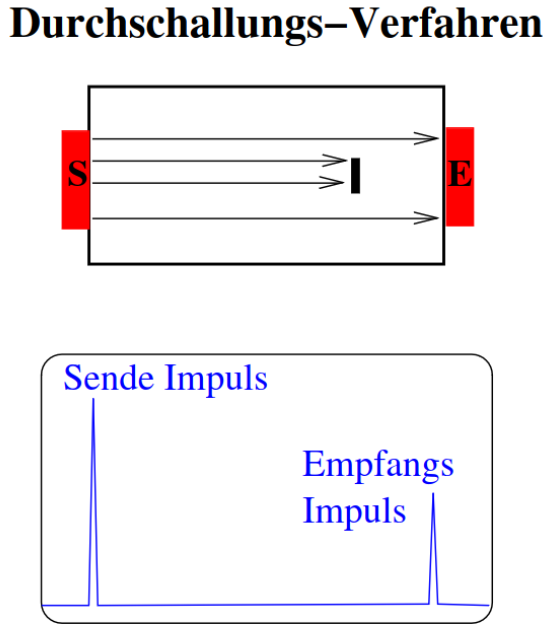
\includegraphics[height=6cm]{Durchschallung.png}
        \caption{Durchschallungs-Verfahren.}
        \label{fig:DSV}
    \end{subfigure}
    \hfill
    \begin{subfigure}{0.48\textwidth}
        \centering 
        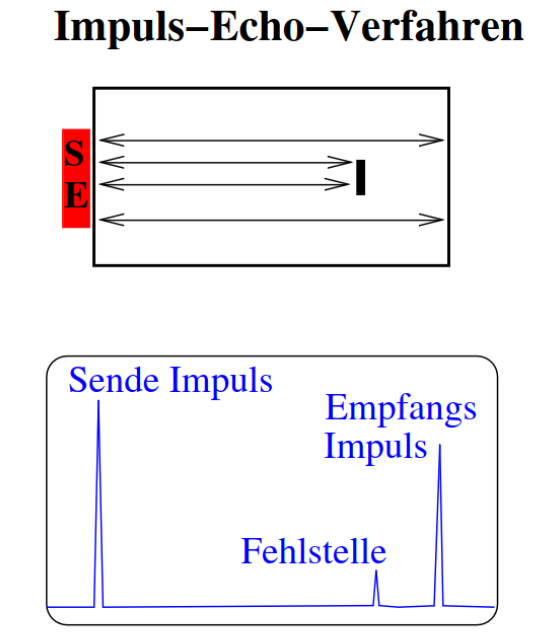
\includegraphics[height=6cm]{Impuls_Echo.png}
        \caption{Impuls-Echo-Verfahren.}
        \label{fig:IEV}
    \end{subfigure}
    \caption{Vergleich beider Verfahren\cite{Versuchsanleitung_US1}.}
    \label{fig:Vergleich}
\end{figure}

\noindent Wie bereits beschrieben, können die Ultraschallergebnisse auf verschiedenen \emph{scans} dargestellt werden.
Der sogenannte \textbf{A-Scan} (Amplituden Scan) ist ein eindimensionales Scan-Verfahren und zeigt die aufgenommenen 
Echoamplituden als Funktion der Laufzeit. Dieses Verfahren wird hauptsächlich zur Abtastung von Strukturen verwendet.
Ein zweidimensionales Schnittbild kann durch den \textbf{B-Scan} (Brightness Scan) erzeugt werden. Wie die Bezeichnung 
bereis vermuten lässt, werden hierbei die Echoamplituden in Helligkeitsstufen unterteilt. Letztlich überbleibt die 
Möglichkeit des \textbf{TM-Scan} (Time-Motion Scan), wobei durch durch schnelles Abtasten eine zeitliche Bildfolge 
aufgenommenen werden kann, um beispielsweise die Bewegung eines Organs darstellen zu können.

\section{Vorbereitung}
Zur Vorbereitung sollen die Schallgeschwindigkeiten c für Luft, Wasser und Acryl recherchiert werden. Es 
lassen sich folgende Werte finden:

\begin{align*}
    c_\text{Luft}   &= \qty{343,2}{\meter \per \second}    \text{\cite{SchallgeschwindigkeitI}}     \\
    c_\text{Wasser} &= \qty{1497}{\meter \per \second}     \text{\cite{SchallgeschwindigkeitI}}    \\
    c_\text{Acryl}  &= \qty{2730}{\meter \per \second}     \text{\cite{SchallgeschwindigkeitII}}    \\
%   c_\text{Aluminium} &= \qty{6320}{\meter \per \second}  \text{\cite{SchallgeschwindigkeitII}}     \\
\end{align*}

\noindent Aus der Schallgeschwindigkeit von Acryl lässt sich nun die frequenzabhängige Wellenlänge berechnen. 
Dazu muss die Schallgeschwindigkeit durch die Frequenz geteilt werden. So ergeben sich für die Frequenz von \qty{2}{\mega\hertz} 
eine Wellenlänge von

\begin{align*}
%    f &= \qty{1}{\mega \hertz} & \Rightarrow& & \lambda_{\qty{1}{\mega \hertz}} &= \qty{2,730}{\milli \meter}   \\
     \lambda &= \qty{1,365}{\milli \meter}   \\
%    f &= \qty{4}{\mega \hertz} & \Rightarrow& & \lambda_{\qty{4}{\mega \hertz}} &= \qty{682,5}{\micro \meter}   \\
\end{align*}

\end{document}